\selectlanguage{english}

\smallframetitle

\section{From 10/06/24 to 14/06/24}
\insertsectionframe

\subsection{Modification of criteria}
\insertsubsectionframe

\begin{frame}{New criteria and city classification}
    After some reflexions, we have agreed to change the way we classify the city-ness of each base station :
    \begin{block}{New city-ness classification}
        \begin{columns}
            \begin{column}{0.4\paperwidth}
                \begin{itemize}
                    \item $d\in\left]0, 1\right]$ : city center;
                    \item $d\in\left]1, 2\right]$ : urban area;
                \end{itemize}
            \end{column}
            \begin{column}{0.4\paperwidth}
                \begin{itemize}
                    \item $d\in\left]2, 4\right]$ : extra-urban area;
                    \item $d\in\left]4, \infty\right[$ : courntryside.
                \end{itemize}
            \end{column}
        \end{columns}
    \end{block}
    \begin{columns}
        \begin{column}{0.4\paperwidth}
            \begin{block}{Angle}
                \begin{itemize}
                    \item $d\in\left]0, 1\right]$ : $\text{angle\_min}=40^\circ$;
                    \item $d\in\left]1, 2\right]$ : $\text{angle\_min}=30^\circ$;
                    \item $d\in\left]2, 4\right]$ : $\text{angle\_min}=25^\circ$;
                    \item $d\in\left]4, \infty\right[$ : $\text{angle\_min}=15^\circ$.
                \end{itemize}
            \end{block}
        \end{column}
        \begin{column}{0.4\paperwidth}
            \begin{block}{Distance}
                \begin{itemize}
                    \item $d\in\left]0, 1\right]$ : $\text{distance\_max}=\unit[2]{km}$;
                    \item $d\in\left]1, 2\right]$ : $\text{distance\_max}=\unit[5]{km}$;
                    \item $d\in\left]2, 4\right]$ : $\text{distance\_max}=\unit[10]{km}$;
                    \item $d\in\left]4, \infty\right[$ : $\text{distance\_max}=\unit[15]{km}$.
                \end{itemize}
            \end{block}
        \end{column}
    \end{columns}
\end{frame}


\subsection{City detection results comparison}
\insertsubsectionframe

\begin{frame}{Reminder : the brute results}
    \begin{figure}
        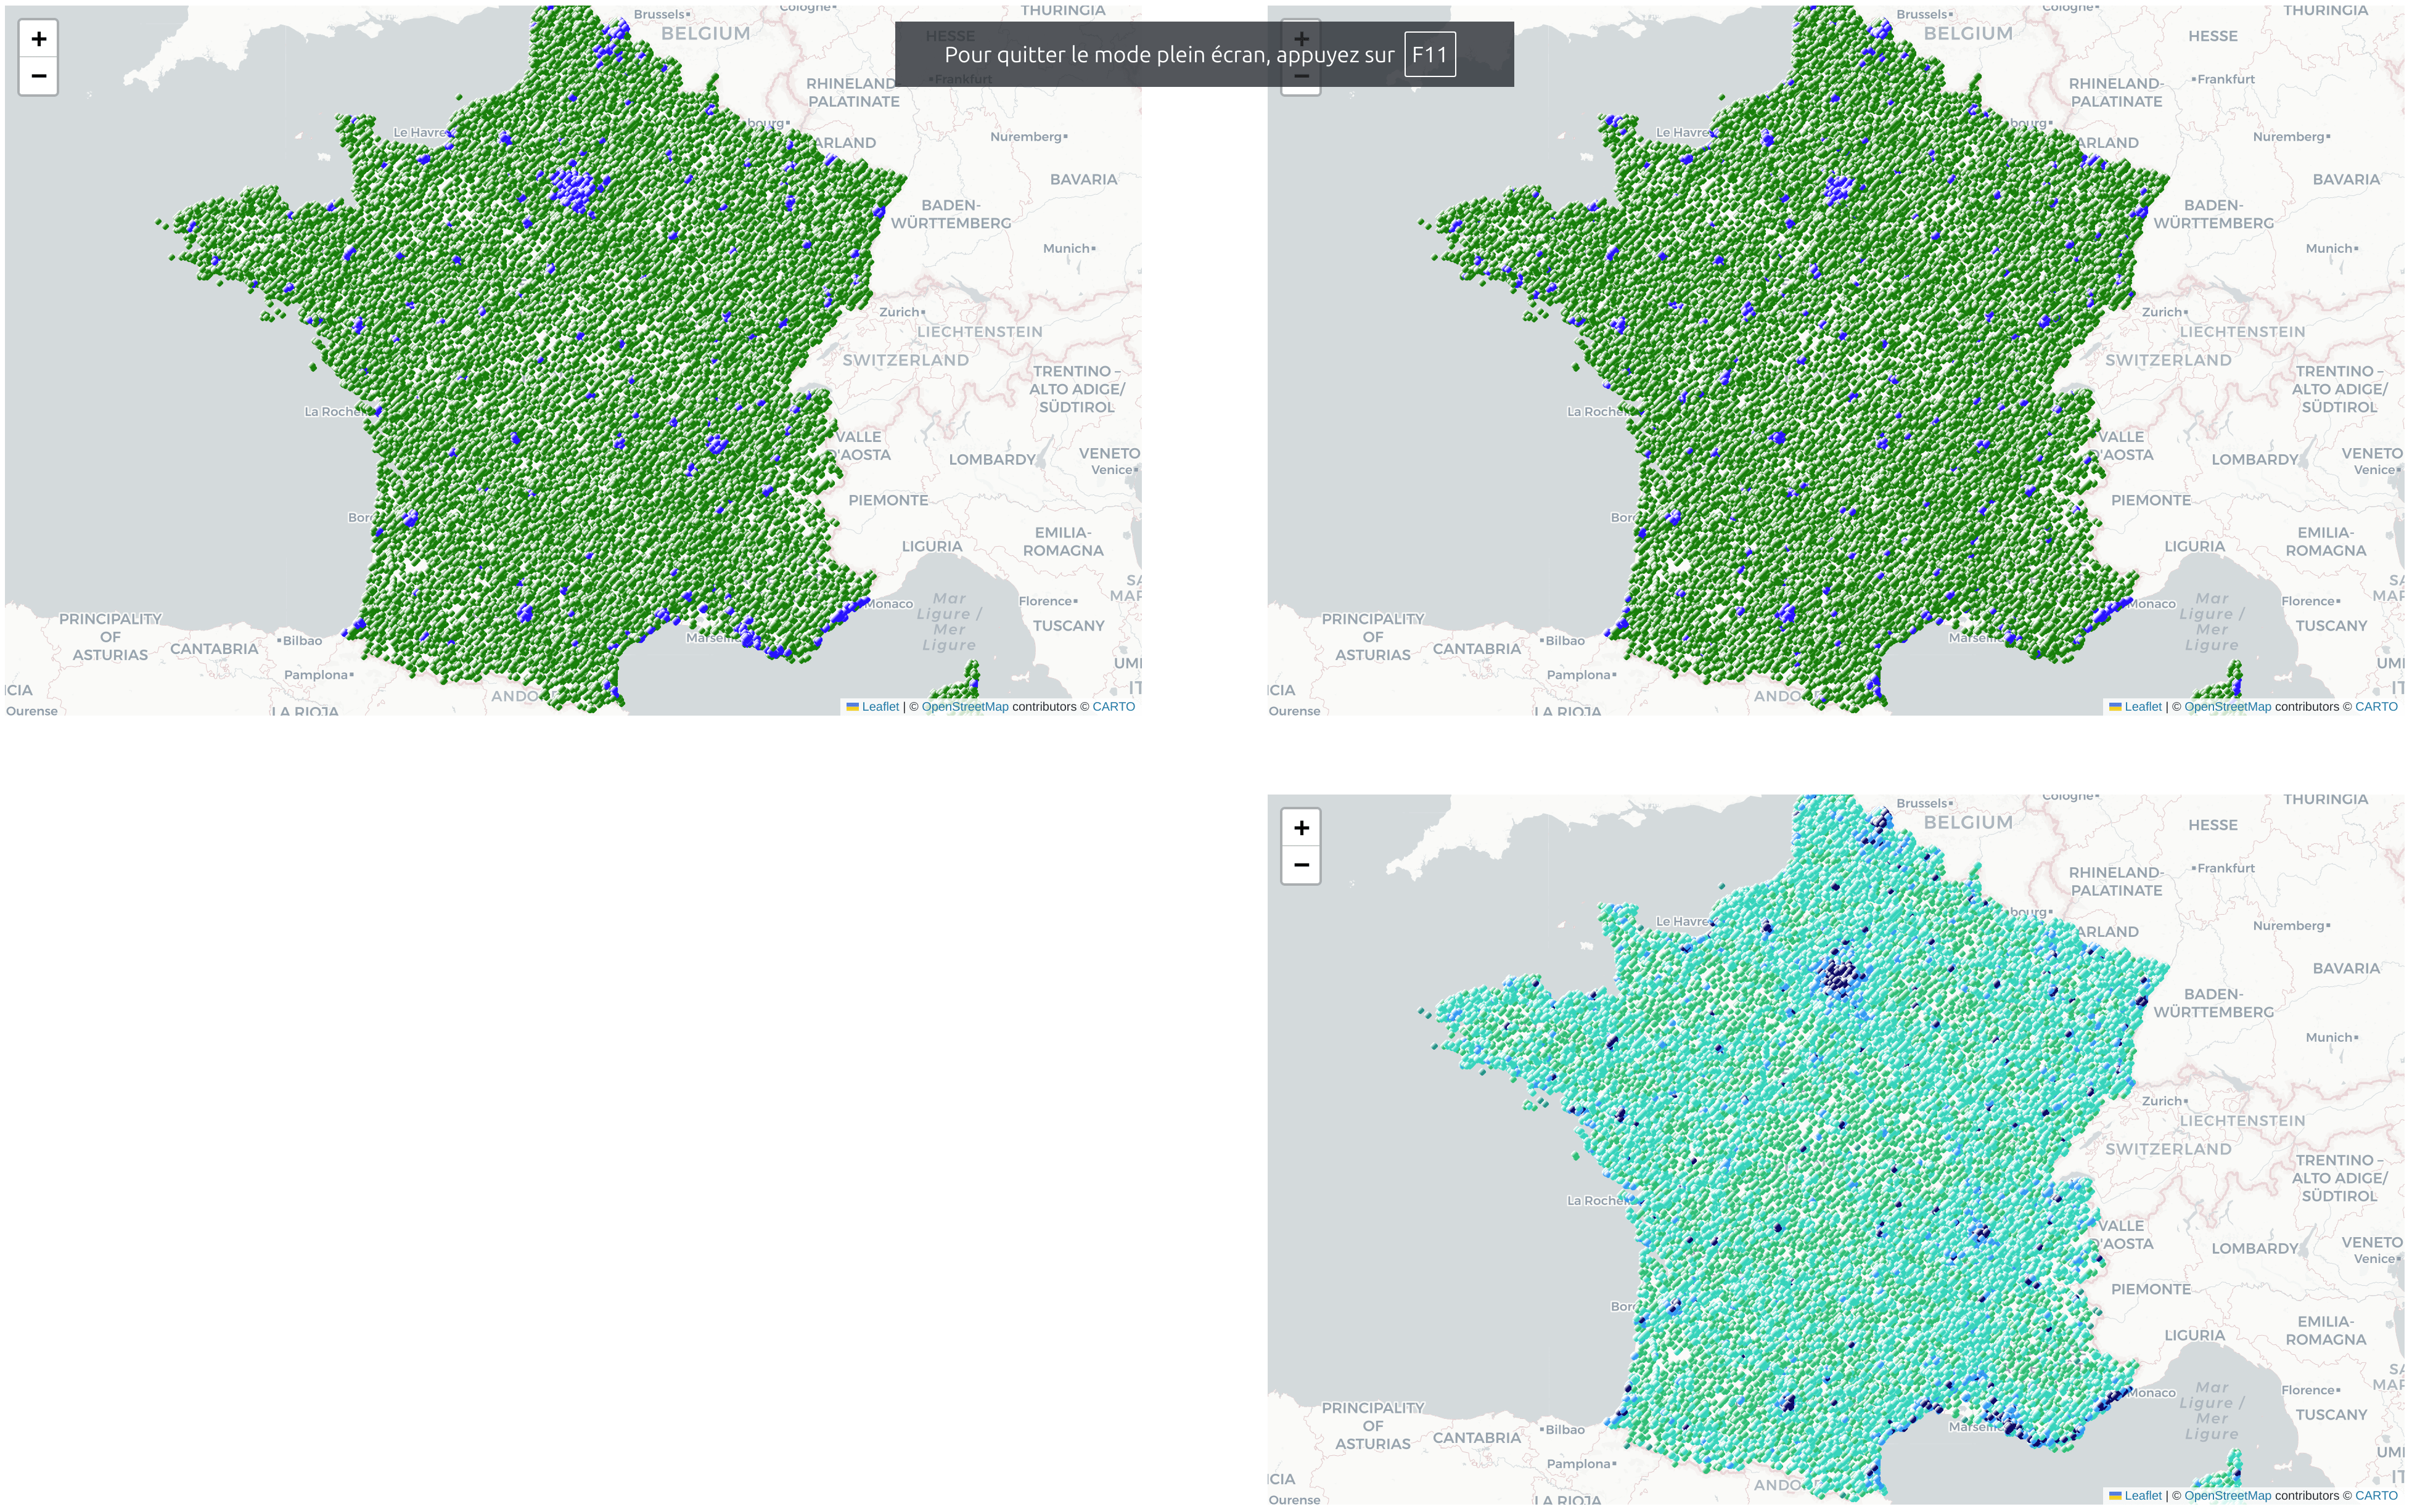
\includegraphics[height=0.6\paperheight]{images/city-detection.png}
        \caption{\label{fig:city-detection}City detection by respectively DBScan, HDBScan and 3-NN methods}
    \end{figure}
\end{frame}

\begin{frame}{Graphical methods comparison}
    \begin{figure}
        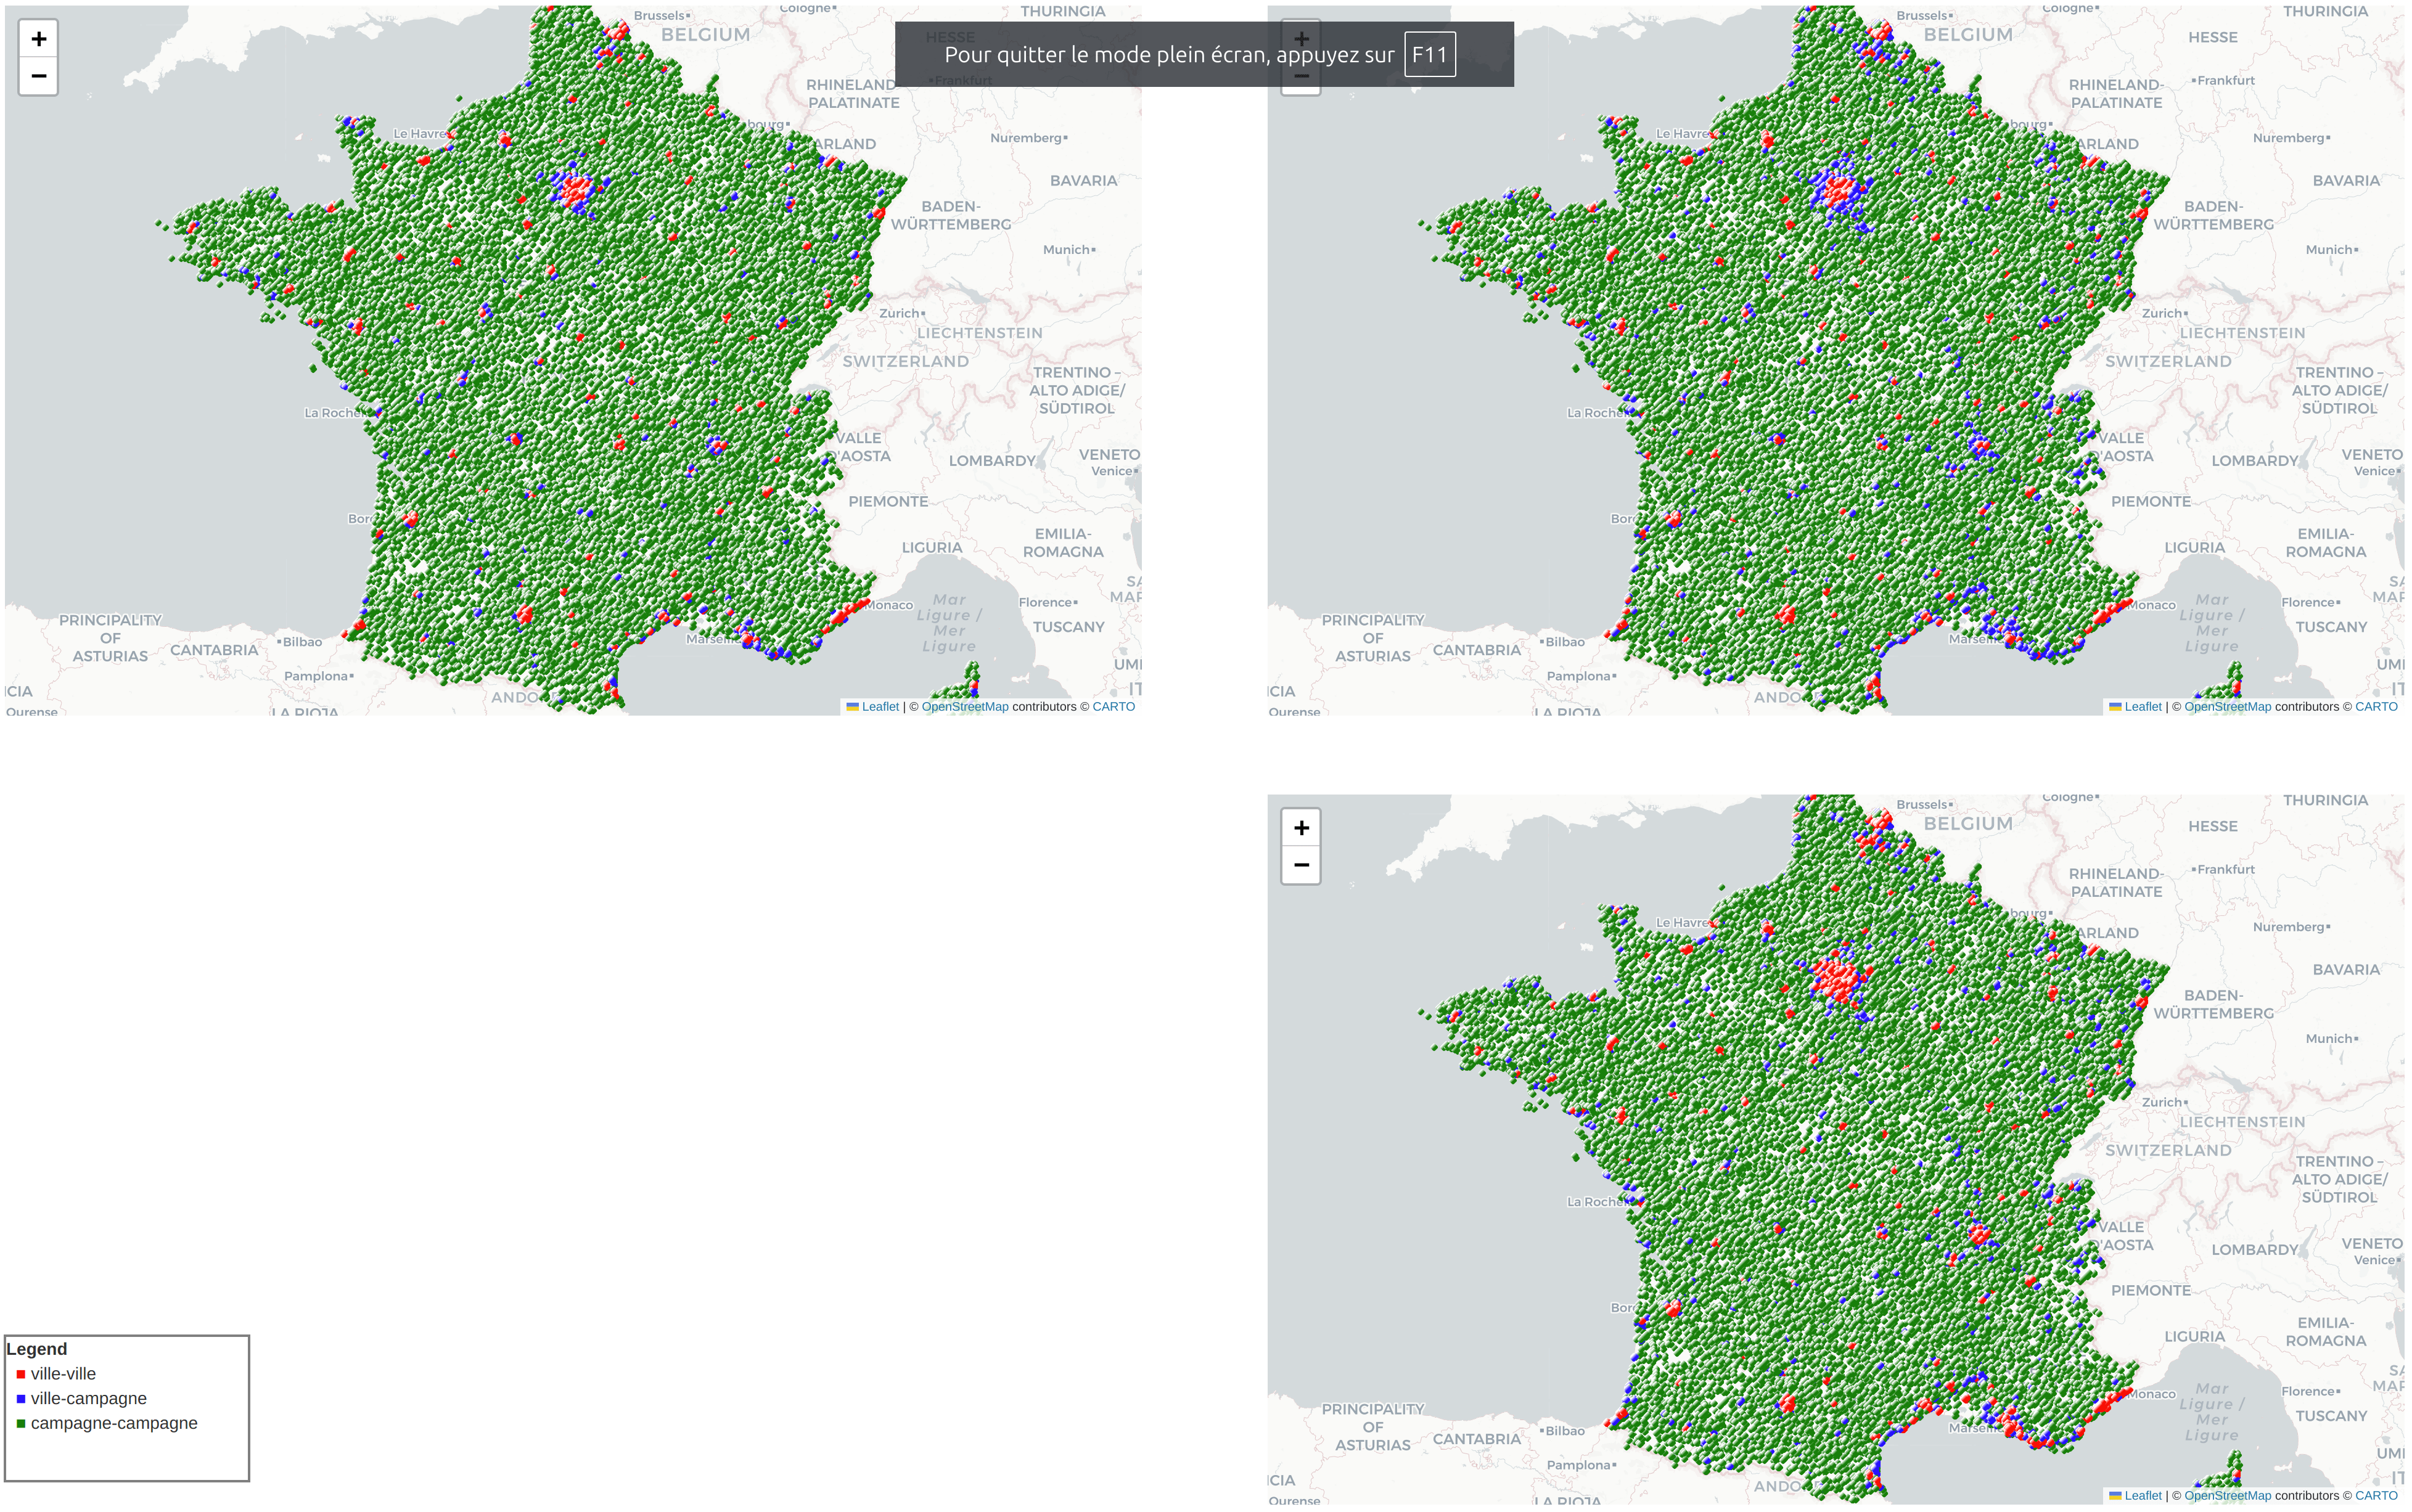
\includegraphics[height=0.6\paperheight]{images/city-detection-comparison.png}
        \caption{\label{fig:city-detection-comparison}DBScan vs HDBScan / HDBScan vs 3-NN / DBScan vs 3-NN}
    \end{figure}
\end{frame}

\begin{frame}{Numerical methods comparison}
    \begin{columns}
        \begin{column}{0.22\paperwidth}
            \begin{block}{DBScan vs HDBScan}
                \begin{itemize}
                    \item $a=0.688$
                    \item $b=0.028$
                    \item $c=0.052$
                    \item $d=0.232$
                \end{itemize}
            \end{block}
        \end{column}
        \begin{column}{0.22\paperwidth}
            \begin{block}{HDBScan vs 3-NN}
                \begin{itemize}
                    \item $a=0.626$
                    \item $b=0.114$
                    \item $c=0.010$
                    \item $d=0.250$
                \end{itemize}
            \end{block}
        \end{column}
        \begin{column}{0.22\paperwidth}
            \begin{block}{DBScan vs 3-NN}
                \begin{itemize}
                    \item $a=0.630$
                    \item $b=0.086$
                    \item $c=0.007$
                    \item $d=0.277$
                \end{itemize}
            \end{block}
        \end{column}
    \end{columns}
\end{frame}

\subsection{Improvement of City detection}
\insertsubsectionframe

\begin{frame}{Reminder : functionnement of base 3-NN}
    \begin{figure}
        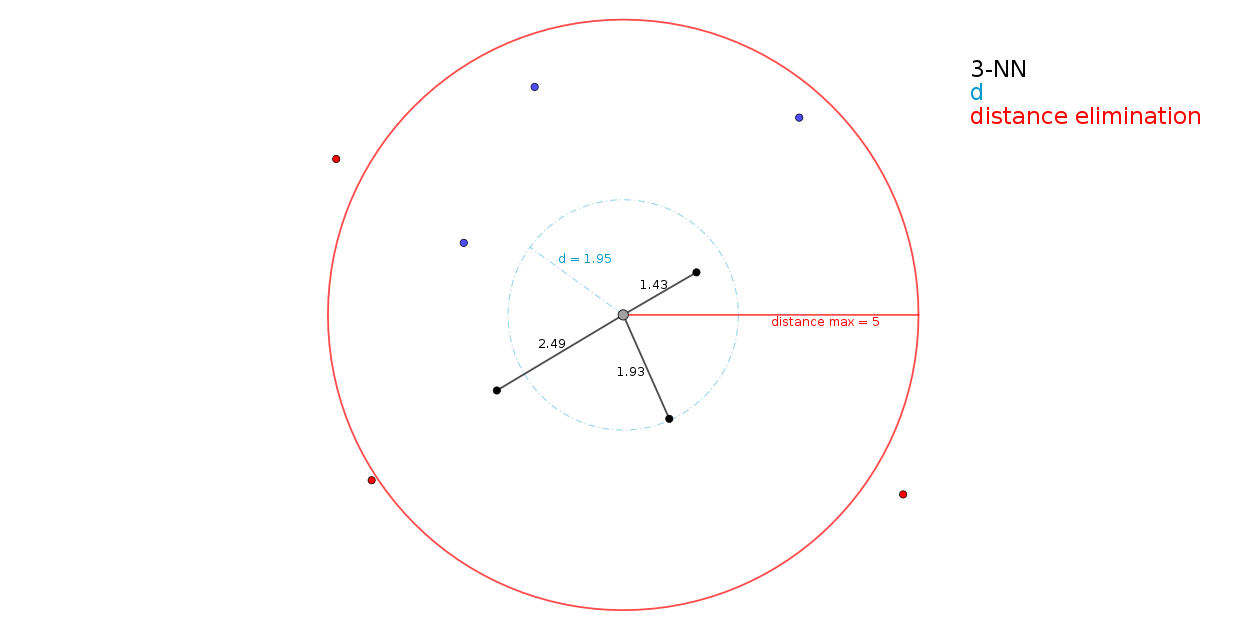
\includegraphics[height=0.6\paperheight]{images/illustration_3-NN.png}
        \caption{\label{fig:illus-3-NN}How 3-NN method works}
    \end{figure}
\end{frame}